
Количественная оценка успеваемости выполняется на основании контрольных работ. Решение об оценки может выноситься как учителем, так и автоматически с использованием приложения. Оценка при обучении выполняют множество задач:
- обучающегося
- оценка перспектив его родителей
- возможность сравнить различные подходы к изложению материала для педагога 


\textit{Определение} \textbf{Психометрия}- дисциплина, изучающая количественные способы оценки знания.

Для этого используются статистические методы оценки знания, учитывающий случайность в измерениях.
Педполагается, что знание не подлежит явному измерению,
а лишь косвенному путем проведения тестирования или анализа деятельности обучающегося.


Для построения теории вводятся скрытые от наблюдения переменные называемыми латентными $\theta$.
В области образования психомтерические исследования наиболее активно выполняются для тестовых заданий. 
Основными подходами к оценке знаний, исходя из результатов, 
на текущий момент является классическая и (item response) теория.

Классическая теория предполагает, что результат тестирования задан случайной величиной. Её вид вид как правило предполагается нормальным:

\begin{equation}
    s \sim \mathrm{N}(\theta,\sigma^2)  
\end{equation}
,где $s$ задает экзаменационный результат обучающегося, параметр $\theta$ - истинный уровень знания, $\sigma^2$ - задает волатильность измерений. распределения с дисперсией, определяемой 

Как правило тесты подбирают таким образом, чтобы ошибка метода на всем промежутке результатов была минимальна
$$
    \int_0^1 \sigma^2(\theta) \rightarrow \min
$$
Существенным недостатком такой системы является предположение о равной сложности задач в контрольной работе.


Система тестирования IRT была предложена институтом в 1950 году. Она активно используется в международных экзаменах языка
и делового знания GMAT и TOEFL

IRT в отличие от классической теории также учитываюет текущий уровень знаний, что позволяет составлять набор заданий индивидуально.
Наиболее известным результатом системы является 3-х параметрическая логистическая модель, учитывающая сложность задачи, вероятность угадать и волатильность оценки Одним из ключевых \cite{lord1956measurement}:
\begin{equation}
    p_i(\theta) = c_i + \frac{1-c_i}{1+e^{-a_i(\theta-b_i)}},
\end{equation}
\begin{figure}[h]
    \centering
    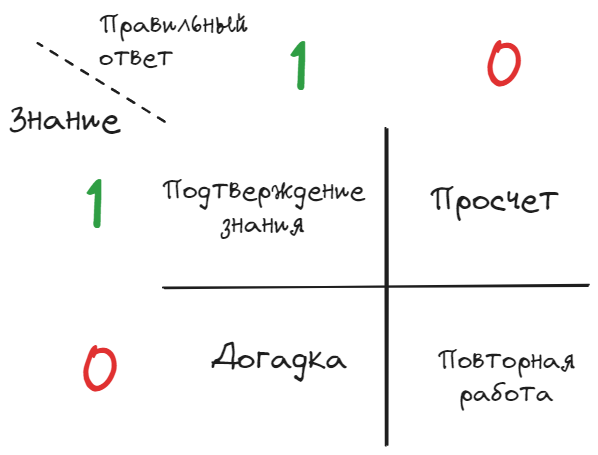
\includegraphics[width=0.5\textwidth]{assets/work/rating/bkt.excalidraw.png}
    \caption{Матрица исходов модели Байесовской оценки на шаге t}
    \label{IRT}
\end{figure}

где коэффициенты \begin{itemize}
    \item $a_i$
    \item $b_i$
    \item $c_i$
\end{itemize}

Альтернативным путем является подход байесовской оценки знания,
описанный в работе \cite{corbett1994knowledge}
\begin{figure}[h]
    \centering
    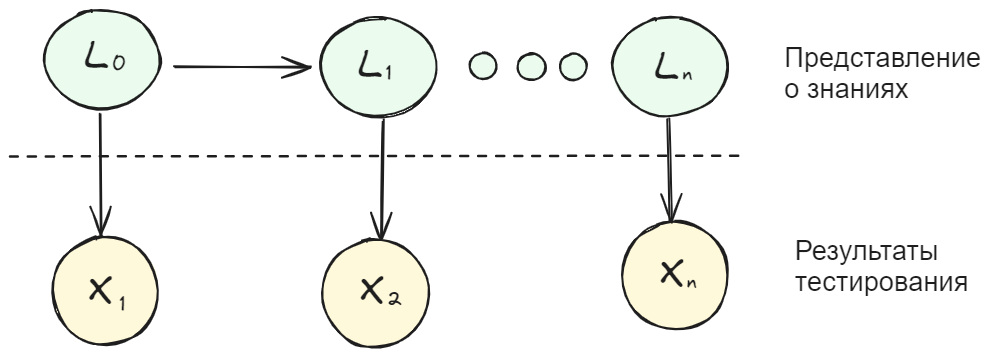
\includegraphics[width=0.5\textwidth]{assets/pedagogic/social/bkt_automata.excalidraw.png}
    \caption{Матрица исходов модели Байесовской оценки на шаге t}
    \label{bkt}
\end{figure}
Задача такой модели подобрать три ключевых параметра \begin{itemize}
    \item $P(L_0)$ начальные знания в предмете
    \item $P(S) = P(x=0| L_t = 1)$ вероятность просчета при наличи знаний
    \item  $P(G) = P(x=1| L_t = 1)$ вероятность угадать при отсутствии знаний
\end{itemize}

При их подборе Байесов подход к оценке позволяет обновлять представления о
степени знаний согласно правилам

\begin{equation}
    \begin{aligned}
        &P(L_t| obs_t=1) = \frac{P(L_t)(1-P(S))}{P(L_t)(1-P(S)) + (1-P(L_t))P(G)} \\
        &P(L_t| obs_t=0) = \frac{P(L_t)P(S)}{P(L_t) P(S) + (1-P(L_t))(1-P(G))}
    \end{aligned}
\end{equation}
Предполагается, что вероятность забыть $ P(L_{t+1}=0|L_t=1)=0$
\begin{equation}
    P(L_{t+1}) = P(L_t|obs_t) + \left(1 - P(L_t | obs_t)\right) P(T)
\end{equation}
Таким, образом тест можно представить в виде марковской цепи обновления представлений о знаниях учащегося \ref{bkt_automata}.
\begin{figure}[h]
    \centering
    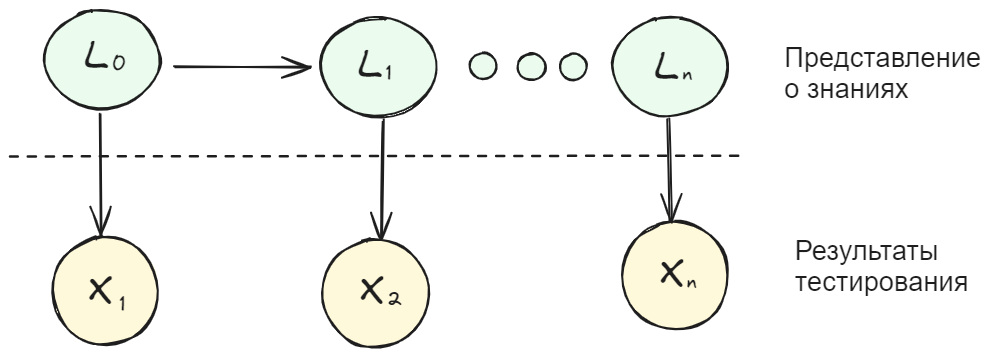
\includegraphics[width=0.5\textwidth]{assets/pedagogic/social/bkt_automata.excalidraw.png}
    \caption{Матрица исходов модели Байесовской оценки на шаге t}
    \label{bkt_automata}
\end{figure}
#Адаптация идеи для случая IRT \ref{IRT} позволяет учесть влияние сложности задания \cite{bulut2023introduction}:
\begin{equation}
    P(Y_{ij}=1| \theta_J, a_i,b_i,c_i) =
\end{equation}


